\documentclass[crop=false, class=memoir]{standalone}

\usepackage[utf8]{inputenc}%Nødvendig for danske bogstaver
\usepackage[danish]{babel}%Sørger for at ting LaTeX gør automatisk er på dansk
\usepackage{csquotes}
\usepackage{geometry}%Til opsætning af siden
\geometry{lmargin = 2.5cm,rmargin = 2.5cm}%sætter begge magner
\usepackage{lipsum}%Fyldtekst, til brug under test af layoutet
\usepackage{float}
\usepackage{graphicx}%Tillader grafik
\usepackage{epstopdf}%Tillader eps filer
\usepackage{marginnote}% Noter i margen
\interfootnotelinepenalty=10000 %undgår at fodnoter bliver spilittet op.
\usepackage[sorting=none]{biblatex}
\addbibresource{litteratur.bib}
\usepackage[hidelinks]{hyperref}%Tillader links
\usepackage{subcaption} % Tillader underfigurer
\usepackage[font={small,sl}]{caption}	% Caption med skrå tekst ikke kursiv

\usepackage{xcolor} %Bruges til farver
\usepackage{forloop} %Bruges til nemmere for loops

\newcounter{opgave}[chapter] %Definerer opgavenumrene og hvornår de nulstilles
\renewcommand{\theopgave}{\thechapter.\arabic{opgave}} %Definerer udseende af opgavenummereringen
\newcounter{delopgave}[opgave] %Definerer delopgavenumrene
\newcounter{lvl} %Definerer en "variabel" til senere brug

\definecolor{markerColor}{rgb}{0.0745098039, 0.262745098, 0.584313725} %Definerer farven af markøren
\newcommand{\markerSymbol}{\ensuremath{\bullet}} %Definerer tegnet for markøren
\newlength{\markerLength} %Definerer en ny længde
\settowidth{\markerLength}{\markerSymbol} %Sætter den nye længde til bredden af markøren

\newenvironment{opgave}[2][0]{%Definerer det nye enviroment, hvor sværhedsgraden er den første parameter med en default på 0
\newcommand{\opg}{\refstepcounter{delopgave}\par\vspace{0.1cm}\noindent\textbf{\thedelopgave)\space}}%Definerer kommando til delopgave
\refstepcounter{opgave}%Forøger opgavenummer med 1 og gør den mulig at referere til
\setcounter{lvl}{#1}%Sætter "variablen" lvl lig med angivelsen af sværhedsgraden
\noindent\hspace*{-0.75em}\hspace*{-\value{lvl}\markerLength}\forloop{lvl}{0}{\value{lvl}<#1}{{\color{markerColor}\markerSymbol}}\hspace*{0.75em}%Sætter et antal af markører svarende til sværhedsgraden
\textbf{Opgave \theopgave : #2}\newline\nopagebreak\ignorespaces}{\bigskip} %Angiver udseende af titlen på opgaverne samt mellemrummet mellem opgaver



\usepackage{mathtools}%Værktøjer til at skrive ligninger
\renewcommand{\phi}{\varphi}%Vi bruger varphi
\renewcommand{\epsilon}{\varepsilon}%Vi bruger varepsilon
\usepackage{physics}%En samling matematikmakroer til brug i fysiske ligninger
\usepackage{braket}%Simplere kommandoer til bra-ket-notation
\usepackage{siunitx}%Pakke der håndterer SI enheder godt
\DeclareSIUnit\clight{\text{\ensuremath{c}}} % Lysets fart i vakuum som c og ikke c_0
\usepackage{chemmacros}
\usechemmodule{isotopes}
\usepackage{tikz}
\usepackage[danish]{cleveref}
\usepackage{nicefrac}
% \renewcommand{\ref}[1]{\cref{#1}}
\creflabelformat{equation}{#2(#1)#3}
\crefrangelabelformat{equation}{#3(#1)#4 to #5(#2)#6}
\crefname{equation}{ligning}{ligningerne}
\Crefname{equation}{Ligning}{Ligningerne}
\crefname{section}{afsnit}{afsnitene}
\Crefname{section}{Afsnit}{Afsnitene}
\crefname{figure}{figur}{figurene}
\Crefname{figure}{Figur}{Figurene}
\crefname{table}{tabel}{tabellerne}
\Crefname{table}{Tabel}{Tabellerne}
\crefname{opgave}{opgave}{opgaverne}
\Crefname{opgave}{Opgave}{Opgaverne}
\crefname{delopgave}{delopgave}{delopgaverne}
\Crefname{delopgave}{Delopgave}{Delopgaverne}

\newcommand{\eqbox}[1]{\begin{empheq}[box=\fbox]{align}
	\begin{split}
	#1
	\end{split}
\end{empheq}}

\newcommand{\kb}{\ensuremath{k_\textsc{b}}}

\DeclareSIUnit{\parsec}{pc}
\DeclareSIUnit{\lightyear}{ly}
\DeclareSIUnit{\astronomicalunit}{AU}
\DeclareSIUnit{\year}{yr}
\DeclareSIUnit{\solarmass}{M_\odot}
\DeclareSIUnit{\solarradius}{R_\odot}
\DeclareSIUnit{\solarluminosity}{L_\odot}
\DeclareSIUnit{\solartemperature}{T_\odot}
\DeclareSIUnit{\earthmass}{M_\oplus}
\DeclareSIUnit{\earthradius}{R_\oplus}
\DeclareSIUnit{\jupitermass}{M_J}

% Infobokse og lignende
% http://mirrors.dotsrc.org/ctan/graphics/awesomebox/awesomebox.pdf
% \usepackage{awesomebox}


% Egen infobokse (virker kun med begrænsede symboler)

\usepackage[framemethod=tikz]{mdframed}
\usetikzlibrary{calc}
\usepackage{kantlipsum}

\usepackage[tikz]{bclogo}

\tikzset{
    % lampsymbol/.style={scale=2,overlay}
    % lampsymbol/.pic={\centering\tikz[scale=5]\node[scale=10,rotate=30]{\bclampe}}.style={scale=2,overlay}
    infosymbol/.style={scale=2,overlay}
}

\newmdenv[
    hidealllines=true,
    nobreak,
    middlelinewidth=.8pt,
    backgroundcolor=blue!10,
    frametitlefont=\bfseries,
    leftmargin=.3cm, rightmargin=.3cm, innerleftmargin=2cm,
    roundcorner=5pt,
    % skipabove=\topsep,skipbelow=\topsep,
    singleextra={\path let \p1=(P), \p2=(O) in ($(\x2,0)+0.92*(1.1,\y1)$) node[infosymbol] {\bcinfo};},
    % singleextra={\path let \p1=(P), \p2=(O) in ($(\x2,0)+0.5*(2,\y1)$) node[infosymbol] {\bcinfo};},
]{info}

% Skal bruges som
% \begin{info}[frametitle={Titel}]
%     Tekst
% \end{info}

\begin{document}

%Inspiration: http://spiff.rit.edu/classes/phys240/lectures/hr/hr.html

\chapter{Stjerner}

\section{Hvad er en stjerne?}

Stjerner er objekter af plasma, som enten sammensætter atomer ved fusion eller har gjort det. De er holdt sammen af deres egen tyngdekraft, og de fleste er i såkaldt \emph{hydrostatisk ligevægt}, hvor tyngdekraften er balanceret med stjernens strålingstryk, således at volumen holdes konstant.

\section{Luminositet, intensitet, flux}
For at diskutere astrofysik, er det nyttigt at kende nogle begreber:

\vspace{1em}
\noindent
\textbf{Luminositet} eller lysstyrke er den totale energi $E$ et objekt udsender i alle retninger per tid $t$.
\begin{align}
    L = \dv{E}{t}
\end{align}
\noindent
\textbf{Flux} beskriver hvor meget af noget man opfanger over et bestemt areal -- sagt med andre ord, hvor meget, der strømmer igennem et areal. Ofte siger man bare flux, når man egentlig mener energiflux -- altså hvor meget af kildens energi vi opfanger. Fluxen $F$ måles i denne sammenhæng som energi $E$ per tid $t$ og areal $A$.
\begin{align}
    F=\frac{1}{A}\pdv{E}{t}
\end{align}
Det svarer til hvor meget af luminositeten, man opfanger over et bestemt areal, fx. på Jorden. Hvis man har et bestemt areal at måle med, og flytter det længere væk fra kilden, bliver det ramt af færre fotoner, så fluxen skal aftage. Fluxen følger
\begin{align}
    F=\frac{L}{4\pi D^2}, \label{stjerner:eq:afstandskv}
\end{align}
hvor $D$ er afstanden til objektet. Dette kaldes \emph{Afstandskvadratloven}, da fluxen falder med kvadratet på afstanden. Så objekter, der er langt væk, ser vi meget svagt. Afstandkvadratloven ser sådan ud, fordi man antager, at stjerner udstråler isotropt, det vil sige lige meget i alle retninger, hvorfor den målte flux i en afstand $D$ fra kilden, er den fra kilden udsendt flux, over hvor stort et areal den har spredt sig over, hvilket er overfladen af en kugle.

\textbf{Intensitet} er et mål for for meget lys der bliver udsendt i en bestemt retning. Det minder om flux, der bare også er divideret med hvor stor en vinkel af himlen man måler på. Vinklen $\dd{\Omega}$ kaldes rumvinklen (``solid angle'' på engelsk). 
\begin{equation}
    I = \frac{\partial^3E}{\partial t \partial A \partial\Omega}
\end{equation}

Det interessante ved intensitet er, at det er uafhængigt af hvor langt man er fra kilden. Afstandskvadratloven siger, at fluxen vil aftage, men til gengæld vil kilden også fylde mindre på himlen, og de effekter opvejer hinanden, så intensiteten bliver konstant.

\section{Størrelsesordenener og enheder indenfor astrofysik}
%Indsæt ordentlig kilde på Alpha Centauri
Det observerbare univers er enormt, og de størrelser, som man arbejder med, er derfor også enorme. Det giver derfor ofte ikke rigtig mening at arbejde med SI-enhederne, som man ellers bruger i det meste andet indenfor fysik. Det er for eksempel en smule uhåndgribelig at tale om, at det nærmeste stjernesystem til vores solsystem ligger \SI{}{\kilo\meter} væk, så giver det bedre mening at sige, at det ligger \SI{4.37}{\lightyear} væk fra os. Ligeledes er det også nemmere at forhold sig til, at Alpha Centauri A har en masse på \SI{1.1}{\solarmass} end at sige, at den har en masse på \SI{}{\kilo\gram}. Nogle af de mest brugte enheder kan ses i \cref{stjerner:tab:enheder}: 

%størrelser fra "Modern Astrophysics"
\begin{table}[H]
\centering
\begin{tabular}{llcS[table-space-text-post = m, table-number-alignment=left, table-format=1.2e2]}\toprule
    Størrelse & "astroenhed" & Symbol & {SI-enhed} \\
    \midrule
    Længde & Jordradius & \si{R_\oplus} & 6.38e6\, \si{\meter}\\
    Længde & Solradius & \si{R_\odot} & 6.97e8\, \si{\meter}\\
    Længde & Astronomisk enhed & \si{\astronomicalunit} & 1.50e11\, \si{\meter}\\
    Længde & Lysår & \si{\lightyear} & 9.46e15\, \si{\meter}\\
    Længde & Parsec & \si{\parsec} & 3.09e16\, \si{\meter}\\
    Masse & Jordmasse & \si{M_\oplus} & 5.97e24\, \si{\kilo\gram}\\
    Masse & Jupitermasse & \si{M_J} & 9.99e99\, \si{\kilo\gram}\\%mangler rigtig værdi
    Masse & Solmasse & \si{\solarmass} & 1.99e30\, \si{\kilo\gram}\\
    Luminositet & Solluminositet & \si{L_\odot} & 3.84e26\, \si{W}\\
    \bottomrule
\end{tabular}
\caption{Enheder, der bruges indenfor astrofysikkens verden i stedet for de standard SI-enheder. Ønskes størrelserne med flere decimaler henvises til tabellen i \cref{mat:sec:fysiskekonstanter}.}
\label{stjerner:tab:enheder}
\end{table}

\section{Rødforskydning}
Du kender nok til, at når en ambulance kører forbi, så lyder sirenens tone højere når den nærmer sig, og dybere når den kører væk. Det skyldes \emph{Dopplerforskydning}, %Find gerne lydklip til undervisningen
%Det skyldes, 
hvilket er en konsekvens af, at lydbølgerne skubbes sammen og strækkes, afhængigt af hvilken fart de udsendes med i forhold til lytteren. Hvis en ambulance kører mod dig, og du står stille, vil du høre bølgerne sammenpresset. Dette skyldes to ting: Først, så er lydens hastighed uændret i mediet. Næst, så bliver lydbølgen udsendt under bevægelse, dvs. at i det tidsrum bølgen bliver sendt ud over, så flytter ambulancen sig også. Derfor vil bølgen virke til at have en kortere bølgelængde, da afstanden har ændret sig under udsendelse (se \cref{stjerner:fig:doppler}).

Men hvis du selv kører med samme hastighed foran ambulancen, så vil du høre dem på samme måde, som de bliver udsendt - altså på samme måde som hvis begge biler står stille, da det er den relative hastighed, som er afgørende.
    
\begin{figure}[H]
	\centering
	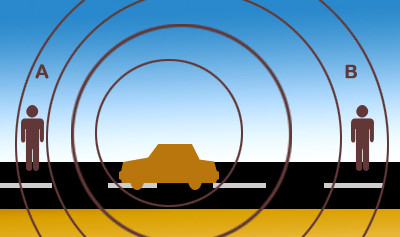
\includegraphics[width=0.7\textwidth]{fig/doppler.jpg}
	\caption{Dopplerforskydning af lyden fra en bil, der kører mod venstre. Person A vil høre en højere tone end person B, og personen i bilen vil høre noget et sted derimellem. Ringene viser et fast punkt på lydbølgerne. Kilde: \cite{DopplerIllustration}.}
	\label{stjerner:fig:doppler} 
\end{figure}
    
Det samme sker for lys. Hvis en ambulance kører væk, vil både tonen af sirenen blive dybere og lyset fra lygterne en smule rødere. Med ``rødere' menes her, at lyset forskydes til at få en længere bølgelængde, og da rødt lys er den del af det visuelle spektrum, der har længst bølgelængder, så vil visuelt lys se rødere ud. Man kalder det derfor også rødforskydning generelt.

Bemærk dog, at selvom fotoner og lydbølger har højere energi ved korte bølgelængder, så mister de ikke energi ved Dopplerforskydning -- der er bare sket et skift i perspektivet, man ser bølgerne fra. Fra bølgens eget synspunkt -- hvis man følger den -- har den samme bølgelængde og energi hele tiden. Der findes også ``kosmologisk rødforskydning'' fra Universets udvidelse, hvor fotonerne rent faktisk mister energi, men dette vil vi ikke beskæftige os med i år.

\section{Spektrum}
Linjer
Absorption og emission, tegn energiniveauer
    
Måden, man måler rødforskydningen på, er ved at opsplitte lyset i dets forskellige bølgelængder. Dvs. man tager spektre af fjerne objekter, og derefter genkender man mønstre fra laboratorier på Jorden. Niels Bohr fik ideen, at elektroner kun kan eksistere i bestemte baner om en atomkerne, men ikke mellem disse. Hver bane har en bestemt energi, så elektronernes energi i atomer er kvantiseret, dvs. de kan kun have den energi, der svarer til lige præcis banernes energier. %findes kun i bestemte pakker. 
Når en elektron henfalder til en lavere tilstand, kommer den af med overskydende energi ved at udsende en foton -- en lyspartikel. Hvis en foton med passende energi rammer en elektron, kan fotonen blive absorberet, så elektronen kommer op i en højere energitilstand. 
    
For lysspektrer gælder 3 love, kaldet Kirchoffs love (ikke at forveksle med Kirchoffs love for elektriske kredsløb), som er illustreret i \cref{stjerner:fig:kirchoff}.
\begin{enumerate}
\item Varme, uigennemsigtige objekter udsender lys kontinuert over hele spektret. Ideelt set ville det give spektret for sortlegemestråling, se \cref{stjerner:sec:sortlegeme}, og det er en særligt god approksimation for varme stjerner. %\emph{Sortlegemestråling} er almindelig stråling som følge af, at objektet er varmt, hvilket beskrives ved en lyskurve, under navnet Planckkurven, som er afhængig af overfladetemperaturen af objektet. Mindre stjernes lys er mere `forurenet' af effekter fra molekylær hydrogen, der er relativt koldt, og andre stoffer. 
%\\Det har vist sig, at en stjernes luminositet, hvis vi antager, at det er et sortlegeme, er relateret til dets radius $R$ og temperatur $T$:
%\begin{equation}
%L = 4\pi\sigma R^2T^4 \propto R^2 T^4
%\end{equation}
%hvor $\sigma$ er Stefan-Boltzmanns konstant. \\
\item Varme, gennemsigte gasser udsender lys, da elektroner exciteres og henfalder, og danner emissionsspektra.
\item Kolde gasser danner absorptionslinjer. Hvis en stjerne ligger bagved og sender lys mod os, vil skyen absorbere lyset og udsende det senere i en tilfældig retning. Dette betyder i længden, at det vil sende lys ud jævnt i alle retninger, hvilket giver en kraftig reduktion i mængden af lys, der når os, da alt lyset pludselig skal fordeles i alle retninger. Så derfor ser vi mindre lys ved denne bølgelængde, end hvis gassen ikke havde været der.
\end{enumerate}

\begin{figure}[H]
	\centering
	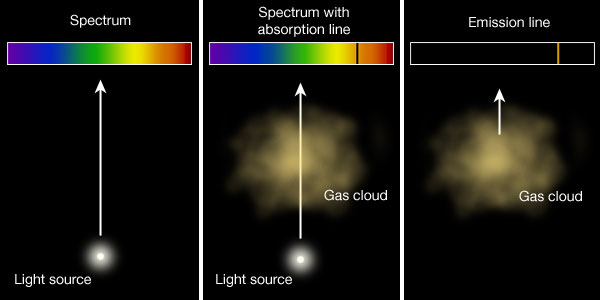
\includegraphics[width=0.6\textwidth]{fig/kirchoffslaws.jpg}
	\caption{Kontinuert spektrum (til venstre), absorptions-spektrum (midtfor) og emissions-spektrum (til højre). Kilde: \cite{AbsorptionEmissionSpectra}.}
	\label{stjerner:fig:kirchoff}
\end{figure}
%fra http://astro.psu.edu/public-outreach/fireworks-masks-1/absorption-and-emission-spectra

\begin{figure}[H]
	\centering
	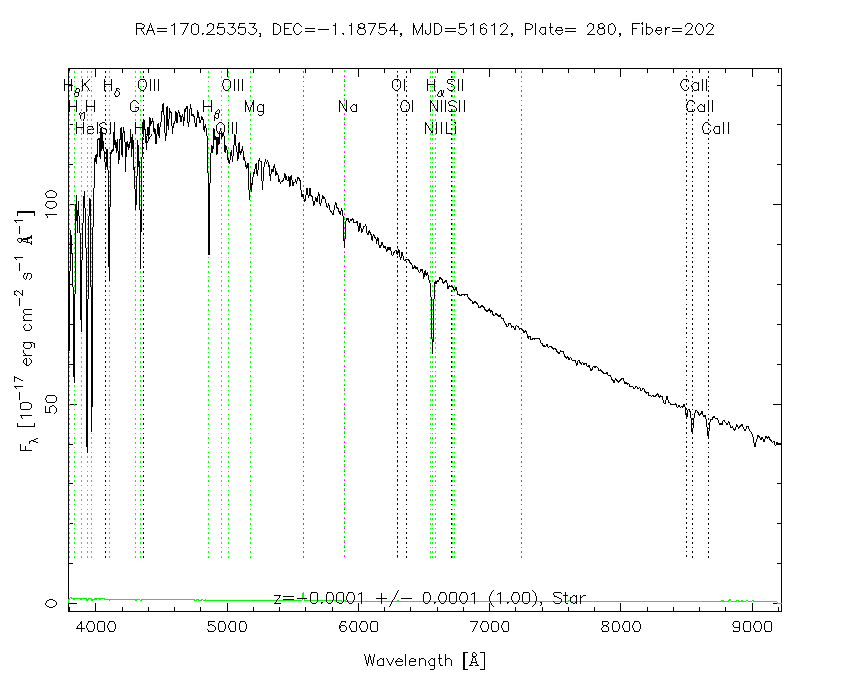
\includegraphics[width=0.6\textwidth]{fig/spektrum.png}
	\caption{Et typisk stjernespektrum. Y-aksen skal forstås som intensitet, mens der	på X-aksen er bølgelængde i ångstrøm (\si{\angstrom}) (\SI{1}{\angstrom} = \SI{e-10}{\meter}). Dykkene i intensitet er angivet med en overgang tilhørende et grundstof, som er identificeret i stjernens atmosfære. Kilde: \cite{Stjernespektrum}.}
    \label{stjerner:fig:spektrum}
\end{figure}
%fra http://i.stack.imgur.com/RMHmB.gif
    
Har man en galakse med en stjerne, som udsender et bredt spektrum af lys, vil lyset både bevæge sig gennem stjernens ydre `kolde' lag og galaksens gasskyer, før det når os. Stjerner og skyer består af forskellige stoffer såsom hydrogen. Når de belyses, absorberer hydrogenet fotoner med de energier, der svarer til energiforskellen mellem banerne i hydrogen. Der dannes derfor et helt bestemt mønster af absorbtionslinjer i spektret, som er unikt for i dette tilfælde hydrogen. For en rødforskudt galakse vil mønsteret ligge ved længere bølgelængder, end det vi måler for hydrogen på Jorden, men det er stadig genkendeligt, som det samme mønster. Et eksempel er vist i \cref{stjerner:fig:spektrum}. 

Når vi kan genkende et mønster af absorptionsliner eller emissionslinjer, selvom det ligger forskudt ved andre bølgelængder end normalt, så kan vi finde rødforskydningen. Den er defineret som forskellen mellem den observeret bølgelængde $\lambda_\text{obs}$ og den i laboratoriet målte bølgelængde $\lambda_\text{lab}$ i forhold til laboratoriebølgelængden (se \cref{stjerner:fig:redshiftmeasure}). Det er altså den relative forskydning i forhold til den oprindelige bølge. Lad os opskrive det som
%
\begin{align}
z=\frac{\lambda_\text{obs}-\lambda_\text{lab}}{\lambda_\text{lab}}. \label{stjerner:eq:redshifty}
\end{align}
%
\begin{figure}
	\centering
	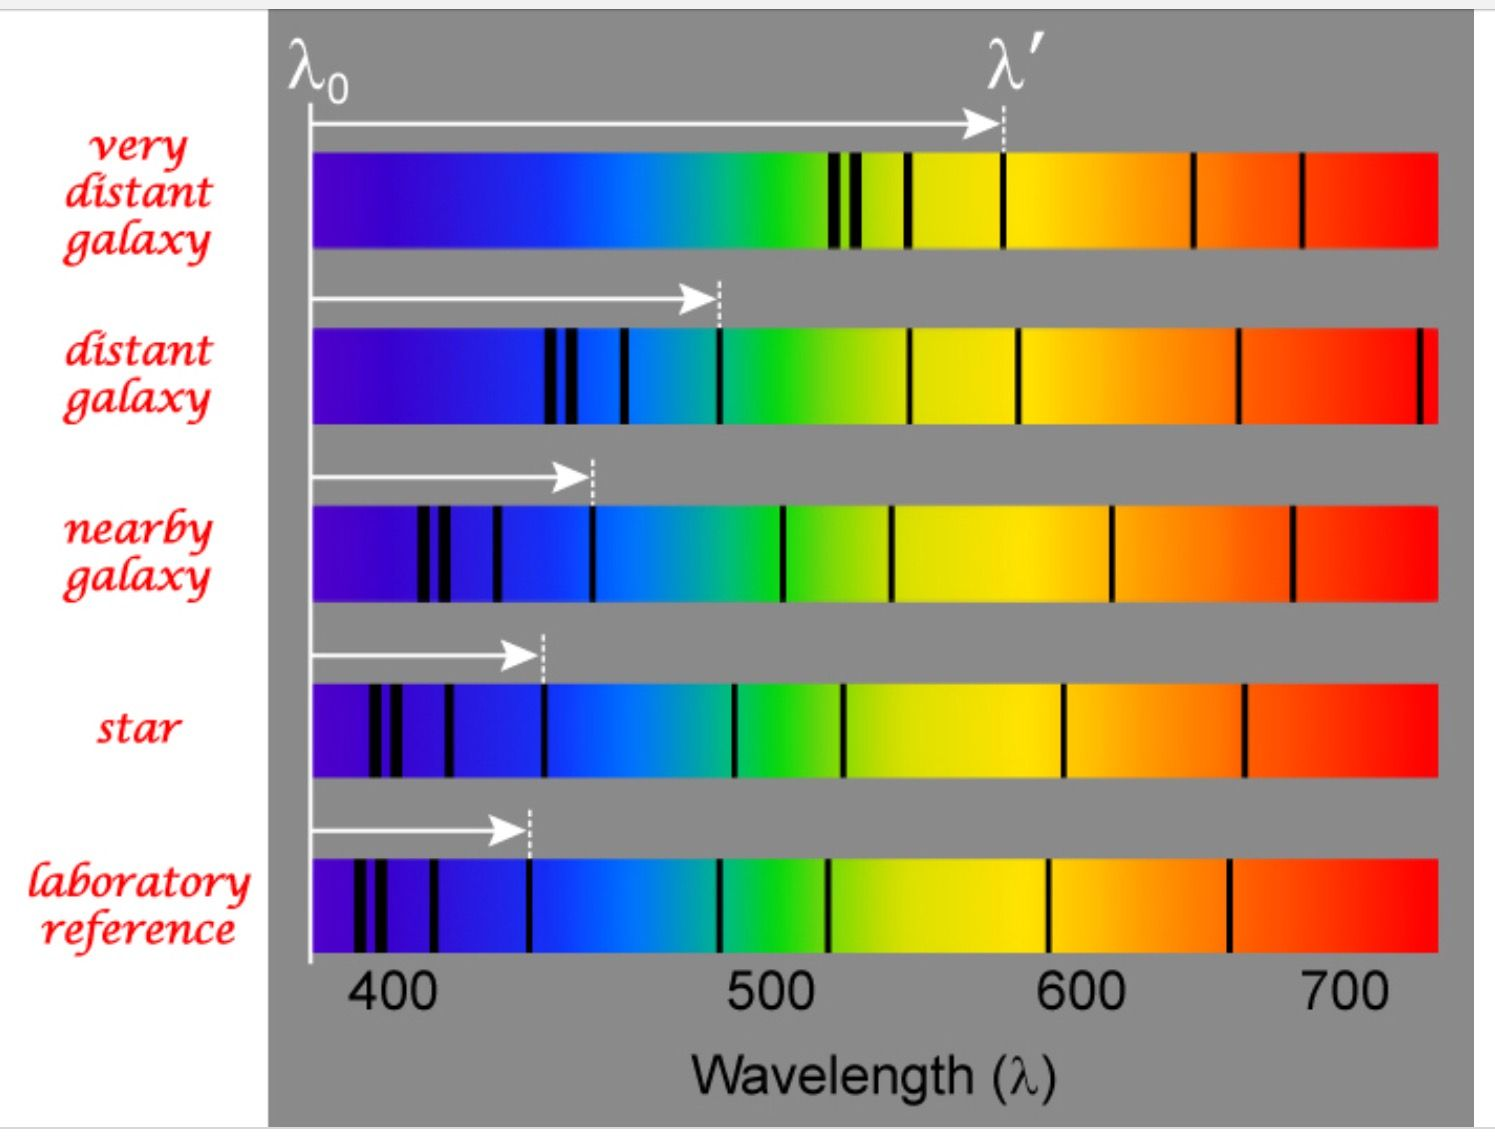
\includegraphics[width=0.6\textwidth]{fig/redshiftcomparison.jpg}
	\caption{\Cref{stjerner:eq:redshifty} bruges ved at måle de indbyrdes forhold mellem absorptionslinjerne i de forskellige spektra. Kilde: \cite{SNC1DEarthSpace}.}
    \label{stjerner:fig:redshiftmeasure}
\end{figure}
%
Rødforskydningen, $z$, er relateret til farten, $v$, således:
\begin{align}
z+1=\sqrt{\frac{1+\frac{v}{c}}{1-\frac{v}{c}}}.
\end{align}
For hastigheder meget langsommere end lysets hastighed i vakuum, $v \ll c$, kan det forsimples til:
\begin{align}
z\approx\frac{v}{c}.
\end{align}
%
%Rødforskydning er altså en form for afstandsmål (da farten, $v$, hænger sammen med afstanden, $D$, ifølge \cref{Hubbleslaw}), men også et tidsmål, da lyset har rejst i lang tid, hvis det har nået at passere en stor afstand og er blevet meget strukket. Hvordan rødforskydningen relaterer til andre måder at måle afstand på, afhænger af hvordan rumtiden strækker lyset. Det kan afgøres af universets form via generel relativitetsteori.
Rødforskydning kan således for eksempel bruges til at bestemme rotationshastigheden for en galakse, da den ene ende vil bevæge sig mod os og den anden ende vil bevæge sig væk fra os\footnote{Det er på denne måde, at man kom på eksistensen af ``mørkt stof'', da man ikke kunne få de målte rotationskurver for galakser til at stemme overens med teorien.}. 

Den kosmologiske rødforskydning kan også bruges til at bestemme afstanden til galakser ved at bruge relationen mellem hastighed ved rødforskydning og afstand, som Hubble og fefef fandt uafhængigt af hinanden og denne relation har fået navnet ``''. Lys fra objekter meget langt væk vil således være mere rødforskudte end galakser tæt på, og da fotonerne fra et objekt langt væk vil have skulle rejse længere tid igennem Universet, vil rødforskydningen af lyset også være et udtryk for alderen af et objekt.

\subsection{Sortlegemespektrum}\label{stjerner:sec:sortlegeme}

Som nævnt i beskrivelsen af Kirchoffs anden lov, så vil varme uigennemsigtige objekter ideelt udsende lys i et kontinuert spektrum, der kaldes for et \emph{sortlegemespektrum}. Sortlegemestråling er stråling, der udsendes fra alle objekter med en temperatur over \SI{0}{\kelvin}. Således udsender både du og kompendiet, som du læser fra, sortlegemestråling, da I begge har en temperatur højere end det absolutte nulpunkt.

Sortlegemestrålingen fra et objekt afhænger af objektets temperatur, og målte man på strålingen ville man få, at den udsendte stråling fordelte sig i en bestem form kaldet en \emph{Planck kurve}\footnote{Den teoretiske udledning af denne form var et af de første skridt i opdagelsen af kvantemekanikken.}. Man ville dog kun få den karakteristiske planck kurve, hvis objektet, man måler, ikke selv udsender nogen anden form for elektromagnetisk stråling. Målte man for eksempel på et spejl, der reflekterede noget lys, ville den målte lyskurve ikke have den karakteristiske form. Således ville man kun få den teoretiske planck kurve fra et objekt, hvis objektet absorberede alt det lys, der ramte det, og udsendte det hele igen som sortlegeme stråling. Sådan et idealiseret objekt kaldes for et \emph{sortlegeme}, heraf navnet sortlegemestråling. Navnet skyldes, at objektet absorberer alt lyset, der rammer det, ligesom sorte objekter absorberer mere af lyset, der rammer det, end hvide objekter gør. Stjerner og planeter kan med gode resultater approksimeres til at være sorte legemer, hvilket gør det nemmere at regne med, og det muliggør at kan sige noget kvantitativt om en stjernes egenskaber baseret på det spektra, som man måler fra stjernen.

Det teoretiske spektrum for sortlegemestrålingen fra et objekt med en temperatur $T$ er givet ved \cref{stjerner:eq:sortlegemestraaling}, og de teoretiske planck kurver for nogle forskellige temperaturer kan ses i \cref{stjerner:fig:planckkurver}. 

\begin{equation}\label{stjerner:eq:sortlegemestraaling}
    B_\lambda(T, \lambda) = \frac{\nicefrac{2hc^2}{\lambda^5}}{e^{\nicefrac{hc}{\lambda\kb T} - 1}}
\end{equation}

Enheden for $B_\lambda(T, \lambda)$ er..... \si{\watt\meter^{-2}\nano\meter^{-1}sr^{-1}}

%Hjemmelavet, placeholder og mangler at blive gjort pænere
% \textwidth = 472.03123pt
\begin{figure}[H]
    \centering
    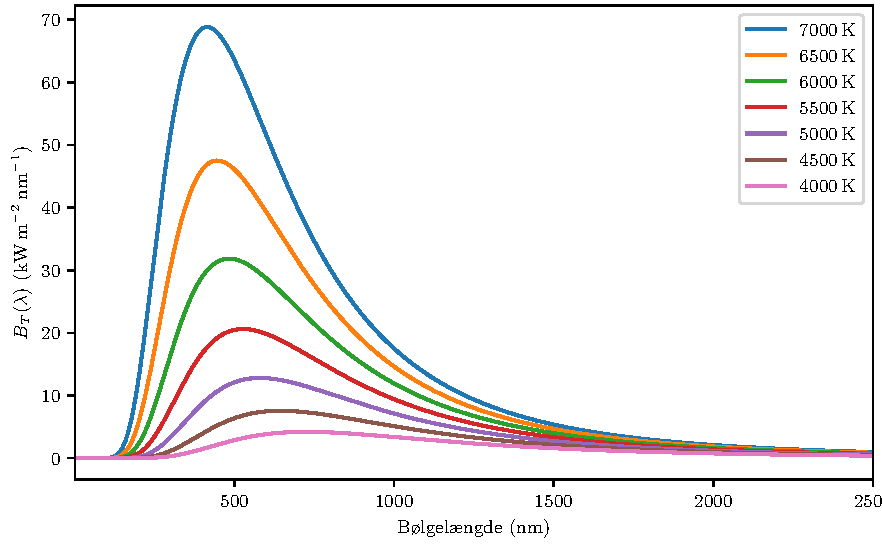
\includegraphics{Stjerner/fig/PlanckKurver.pdf}
    \caption{Sortlegemespektra for objekter med en temperatur på \SIrange{4000}{7000}{\kelvin}. Det kan ses, at kurvernes toppunkter ligger ved lavere bølgelængder for højere temperaturer. %Det markerede område viser det udsnit af spektrummet, der passer med det synlige spektrum.
    }
    \label{stjerner:fig:planckkurver}
\end{figure}

Det kan ses på kurverne i \cref{stjerner:fig:planckkurver}, at et objekt med en højere temperatur vil udsende elektromagnetisk stråling med en højere intensitet ved de lavere bølgelængder og toppunktet for kurven er også forskudt mod de lavere bølgelængder.

Placeringen af toppunktet for spektrummet kan med en approksimation bestemmes ved at bruge  \emph{Wiens~forskydningslov}, som kan ses i \cref{stjerner:eq:wienslov}:
\begin{equation}\label{stjerner:eq:wienslov}
    \lambda_\text{max} = \frac{\SI{0.002897755}{\meter\kelvin}}{T}
\end{equation}

Fysikerne Josef Stefan og Ludwig Boltzmann viste i sin tid, at luminositeten af et sortlegeme kun afhang af dets overfladeareal. Antages det, at stjerner fungerer som sortelgemer, så kan overfladearealet af en kugle indsættes for arealet, og man får \emph{Stefan-Boltzmanns ligning}, se \cref{stjerner:eq:stefanboltzmannligning}, hvor $\sigma \approx \SI{5.67e-8}{\watt/(\meter^2\kelvin^4)}$ er \emph{Stefan-Boltzmanns konstant}:

\begin{equation}\label{stjerner:eq:stefanboltzmannligning}
    L = 4\pi\sigma R^2 T^4
\end{equation}

Herved har man en ligning, hvor man kan bestemme enten temperaturen, radius eller luminositeten af en stjerne, hvis man kender de to andre størrelser. Har man således bestemt afstanden til en stjerne med parallakse metoden, så man kan bestemme dens luminositet, sammen med, at man har fundet dens temperatur ved at se på dens spektrum, så kan man bruge disse informationer til at bestemme størrelsen af stjernen.

\section{Afstand}
Afstand er et vigtigt begreb i astrofysikken, men ofte også svært at måle. Derfor har vi mange forskellige typer af afstandsmål, og hvordan de hænger sammen, er ikke altid fastlagt. En af de mest brugte metoder til bestemmelse af afstande er gennem et objekts \emph{luminositet}. 

Fra introduktionen kan vi huske, hvis et objekts energi er udsendt uniformt i alle retninger og modtages i en afstand $D$ væk, var den modtagende \emph{tilsyneladende luminositet} -- eller \emph{flux} -- givet ved \cref{stjerner:eq:afstandskv}. Fra den ligning kan man isolere et udtryk for afstanden:
\begin{equation} \label{stjerner:eq:L}
D = \sqrt{\frac{L}{4\pi F}}
\end{equation}

Ved man således, hvor lysstærk en stjerne burde være, kan man sammenligne det med den flux, som man måler og på den måde bestemme afstanden. 

Ekstinktion?



\subsection{Parallakse}
Lysår, AU, ’’, pc
D\_P=1/theta[’’] *pc 

En anden metode, der er god til at måle afstande til nære stjerner, er ``parallakse-metoden''. Denne er mere lavpraktisk end den forrige metode, da denne metode for eksempel ikke kræver viden om den målte stjernes luminositet. 

%Placeholder figur indtil videre
\begin{figure}[H]
    \centering
    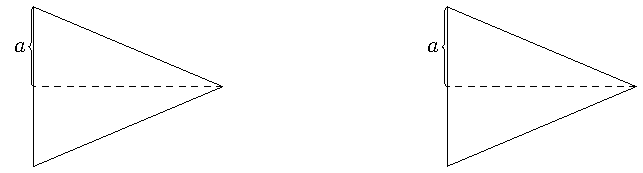
\includegraphics{fig/Parallakse.pdf}
    \caption{Caption}
    \label{stjernerfig:parallakse}
\end{figure}{}


\begin{equation}
    D_P = \frac{1}{\theta}
\end{equation}



\section{Magnitude}

Indenfor astronomiens verden beskrives et objekts lysstyrke ved \emph{magnitudesystemet}. Dette er et logaritmisk system, der rækker helt tilbage til Hipparchos i antikkens Grækenland. Af historiske årsager fungerer systemet således, at jo højere magnitude, desto svagere ser objektet ud på himlen og omvendt. Dengang fandtes der ikke teleskoper, som i dag, så alle målinger af stjerner blev taget per øjemål. Dengang gik skalaen fra 0 til og med 6, hvor 0 var det stærkeste på himlen og så fremdeles. Vi bruger i dag en skala, der er defineret således, at grækernes målinger stadig passer ind. Den tilsyneladende magnitude af et objekt vil variere med afstanden -- hvis man flytter sig tættere på en stjerne, vil den få en lavere magnitude (svarende til højere lysstyrke). Hvis man tager højde for afstanden, får man objektets absolutte magnitude, der er ens for alle observatører.
    
Den tilsyneladende magnitude af et objekt kan bruges til at bestemme afstanden ved at bruge
\begin{equation}
m-M=5\cdot \log_{10}\left(\frac{d_L}{\SI{1}{\parsec}}\right) - 5 ,
\end{equation}
hvor $m$ er den tilsyneladende magnitude, $M$ er den absolutte magnitude, og $d_L$ er afstanden til objektet målt i parsec ([pc]). Forskellen kaldes objektets distancemodulus. Når der divideres med parsec, så er det blot for at fjerne længdeenheden, da man kun kan tage logaritmen til et tal uden enhed.

\section{HR-diagram}

Et Hertzsprung-Russell diagram, forkortet ``HR-diagram'', er et diagram, hvor man har indsat stjerners luminositet som funktion af deres temperatur. Diagrammet er opkaldt efter ... og ..., der hver især fik den samme ide til at lave sådan et diagram.

\section{Stjernetyper (OBAFGKMLT, neutron, dværge, kæmper, superkæmper)}
Formel for overfladetemperatur (R,T,L)
Bånd og hvad er de gode til?
Farvediagrammer

\begin{equation}
    T = \sqrt[4]{\frac{L}{4\pi\sigma R^2}}
\end{equation}

\section{Udvikling}
Dannelse
Stjernesystemer
Kerneprocesser
PP og CNO
s og r
Supernovaer

\subsection{Kerneprocesser}

\textbf{PP I chain} \cite{CarrolOstlieModernAstrophysics2017}
    
\begin{align}
    \isotope{H} + \isotope{H} &\rightarrow \isotope{2,H} + e^+ + \gamma\\
    \isotope{2,H} + \isotope{H} &\rightarrow \isotope{3,He} + \gamma\\
    \isotope{3,He} + \isotope{3,He} &\rightarrow \isotope{He} + 2\, \isotope{H}
\end{align}
    
\textbf{PP II chain}
    
\begin{align}
    \isotope{3,He} + \isotope{He} &\rightarrow \isotope{7,Be} + \gamma\\
    \isotope{7,Be} + e^- &\rightarrow \isotope{Li} + \nu_e\\
    \isotope{Li} + \isotope{H} &\rightarrow 2\, \isotope{He}
\end{align}
    
\textbf{PP III chain}

\begin{align}
    \isotope{7,Be} + \isotope{H} &\rightarrow \isotope{8,B} + \gamma\\
    \isotope{8,B} &\rightarrow \isotope{8,Be} + e^+ + \nu_e\\
    \isotope{8,Be} &\rightarrow 2\, \isotope{He}
\end{align}
    
\textbf{CNO cycle}
    
\begin{align}
    \isotope{C} + \isotope{H} &\rightarrow \isotope{13,N} + \gamma\\
    \isotope{13,N} &\rightarrow \isotope{13,C} + e^+ + \nu_e\\
    \isotope{13,C} + \isotope{H} &\rightarrow \isotope{N} + \gamma\\
    \isotope{N} + \isotope{H} &\rightarrow \isotope{15,O} + \gamma\\
    \isotope{15,O} &\rightarrow \isotope{15,N} + e^+ + \nu_e\\
    \isotope{15,N} + \isotope{H} &\rightarrow \isotope{C} + \isotope{He}
\end{align}

\subsection{Stjerners endeligt}

Stjerner ender på forskellige måder blablabla....

\begin{itemize}
    \item \textbf{Hvide dværge:}
    \item \textbf{Supernovaer:}
    \item \textbf{Neutron stjerner:}
    \item \textbf{Kilonovaer:}
    \item \textbf{Sorte huler:}
\end{itemize}

\subsection{S- og r-processer}

``Slow-process'' ``Rapid-process''

\section{IMF}

(engelsk: ``Initial Mass Function'')

\section{Kriterie for stjernekollaps}

Hvad skal der til for at der sker et kollaps????????

\subsection{Virial teoremet}

\begin{equation*}
    2K + U = 0
\end{equation*}

\subsection{Jeans masse}

\begin{align*}
    U &\sim -\frac{3}{5}\frac{GM_c^2}{R_c}\\
    K &= \frac{3}{2}N\kb T\\
    N &= \frac{M_c}{\mu m_H}\\
    2K &< \abs{U}\\
    \frac{3M_c \kb T}{\mu m_H} &< \frac{3}{4} \frac{GM_c^2}{R_c}\\
    R_c &= \qty(\frac{3M_c}{4\pi \rho_0})^{1/3}\\
    M_c &> M_J\\
    M_J &\simeq \qty(\frac{5\kb T}{G\mu m_H})^{\nicefrac{3}{2}}\qty(\frac{3}{4\pi\rho_0})^{\nicefrac{1}{2}}\\
    R_J &\simeq \qty(\frac{15\kb T}{4\pi G\mu m_H \rho_0})^{\nicefrac{1}{2}}
\end{align*}

\section{Hydrostatisk ligevægt}
%Udled det
%Transport af stråling, energi og temperatur

Som der stod i introduktionen til dette hovedemne, så er de fleste stjerner i noget, der kaldes for \emph{hydrostatisk ligevægt}. 

\begin{align}
    dm \dv[2]{r}{t} &= F_g + F_{P,t} + F_{P,b}\\
    F_{P,t} &= -(F_{P,b} + dF_P)\\
    dm \dv[2]{r}{t} &= F_g - dF_P\\
    F_g &= -G \frac{M_rdm}{r^2}\\
    P \equiv \frac{F}{A}\\
    dF_P &= A dP\\
    dm \dv[2]{r}{t} &= -G \frac{M_r dm}{r^2} - A dP\\
    dm &= \rho A dr\\
    \rho A dr \dv[2]{r}{t} &= -G \frac{M_r \rho A dr}{r^2} - A dP\\
    \rho \dv[2]{r}{t} &= -G \frac{M_r \rho}{r^2} - \dv{P}{r}\\
    \dv[2]{r}{t} &= 0\\
    \dv{P}{r} &= -G\frac{M_r\rho}{r^2} = -\rho g
\end{align}

\subsection{Andre tilstandsligninger}

\begin{align}
    \dv{M_r}{r} &= 4\pi r^2 \rho\\
    \dv{L_r}{r} &= 4\pi r^2 \rho \epsilon
\end{align}

\section{Lane-Emden eq (kun hvis der er plads)}

\begin{equation}
    \frac{1}{\xi^2} \dv{\xi}(\xi^2\dv{\theta(n)}{\xi}) = -\theta(n)^n
\end{equation}

\section{Mål i grupper på noget der ikke er Saturn - vi laver random grupper}

\section{Observationelle ting}
Data processing


\end{document}